\HeaderQuote{What is the use of a book, without pictures or conversations?}{Alice} 

\chapter{Something different }

\FirstSentence{O}{ff with their head!} \lipsum[1]
\begin{equation}
    \zeta = \frac{1039}{\pi}
\end{equation}

\section{Cleverref}
For an example of a full page figure, see \cref{fig:myFullPageFigure}. 
\Cref{fig:teaparty} on the other hand is a smaller figure, inline with text. 
The \texttt{cleverref} package is very convenient, as it uses the same 
formatting throughout, i.e., not \emph{Figure} vs. \emph{figure} 
inconsistencies. You can also refer to your papers, e.g. 
\cref{InRu11a}\footnote{Update \texttt{endmatter/papers.tex},
    \texttt{frontmatter/papers.tex} and \texttt{papers/papers.bib} to your 
    publications.},  
with their roman numeral. Always calling \texttt{$\backslash$cref}.

\lipsum[3]

\section{First Paragraph}
And now I begin my first chapter here ...

Here is an equation\footnote{the notation is explained in the nomenclature 
section}:
\begin{eqnarray}
	CIF: \hspace*{5mm}F_0^j(a) &=& \frac{1}{2\pi \iota} \oint_{\gamma} \frac{F_0^j(z)}{z - a} dz
\end{eqnarray}

\lipsum[4-6]

You can also include pseudocode, such as in \cref{pseudo:example}.
\lipsum[4-6]

% Package Documentation: 
%http://ctan.mirrorcatalogs.com/macros/latex/contrib/algorithmicx/algorithmicx.pdf

\begin{algorithm}[t]
    \caption{Euclid's algorithm}\label{pseudo:example}
    \begin{algorithmic}[1]
        \Procedure{Euclid}{$a,b$}\Comment{The g.c.d. of a and b}
        \State $r\gets a\bmod b$
        \While{$r\not=0$}\Comment{We have the answer if r is 0}
        \State $a\gets b$
        \State $b\gets r$
        \State $r\gets a\bmod b$
        \EndWhile\label{euclidendwhile}
        \State \textbf{return} $b$\Comment{The gcd is b}
        \EndProcedure
    \end{algorithmic}
\end{algorithm}

\section{Mad Hatter's Tea Party}
There are many examples of Job-Shop Scheduling Problem (JSP) for real-world 
application. 
However, for demonstration purposes, let's examine a hypothetical problem from 
the 18th century. 
Assume we are invited to the Mad Hatter's Tea Party in Wonderland 
illustrated in \cref{fig:teaparty}. 
There are four guests attending, namely
\begin{enumerate*}[label={$J_\arabic*$)}, ref={{$J_\arabic*$}}, 
    itemjoin*={{, and of course our host }}]
    \item Alice\label{guest:alice}
    \item March Hare\label{guest:marchhare}
    \item Dormouse\label{guest:dormouse}
    \item Mad Hatter\label{guest:madhatter}
\end{enumerate*}
During these festivities, there are several things each member of the party 
has to perform. They all have to
\begin{enumerate*}[label={$M_\arabic*$)}]
    \item have wine or pour tea
    \item spread butter
    \item get a haircut
    \item check the time of the broken watch for themselves
    \item say what you mean, be it asking a riddle, telling a story, or singing 
    a song to the group
\end{enumerate*}
Our guests are very particular creatures, and would like to do these task in a 
very specific order, e.g., March Hare insists on doing 
them in alphabetical order. And each would rather wait than breaking their 
habit.
Moreover, they tend to be very absent-minded so each task takes them a 
different amount of time. 
Let's assume that their processing times and ordering are given in 
\cref{tbl:example}. 

\begin{figure}[b!]\centering 
    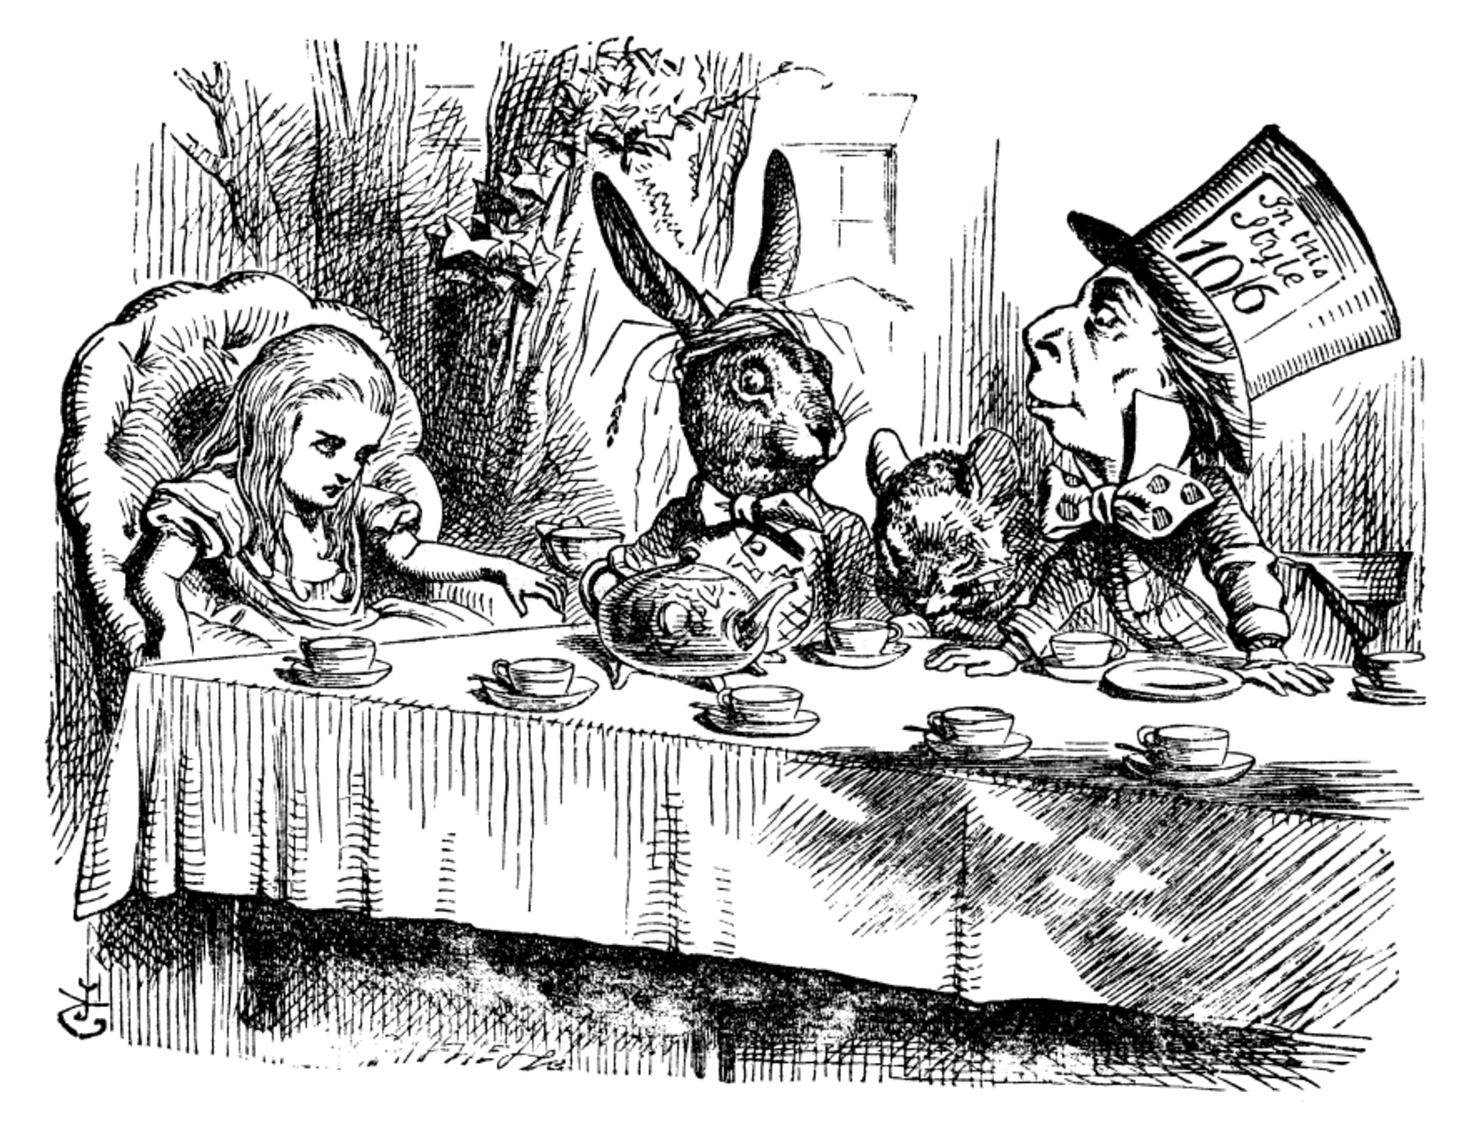
\includegraphics[width=0.8\textwidth]{alice-mad-tea-party}
    \caption[Short figure name.]{The Mad Hatter's Tea Party, from Alice's 
    Adventures in Wonderland by \citet{alice}. 
    Illustration by John Tenniel (1820-1914).}\label{fig:teaparty}
\end{figure}

\begin{table}[t!]\centering
%j.rnd.4x5.train.csv => instance problem.1
\caption{Example of $4\times5$ \JSP}\label{tbl:example}
\begin{tabular}{lc|ccccc|ccccc} \toprule
Guest & \multicolumn{1}{c}{Job} & \multicolumn{5}{c}{Machine ordering 
$\vsigma$} & \multicolumn{5}{c}{Processing times $\vec{p}$} \\ \midrule
%0 16 1 5 2 10 3 15 4 10 
Alice & \ref{guest:alice} & \st{1} & \st{2} & \st{3} & \st{4} & 
\st{5} & 
\st{26} & \st{25} & \st{40} & \st{15} & \st{42} \\
%0 18 1 16 2 36 3 68 4 44 
March Hare & \ref{guest:marchhare} & \st{1} & \textbf{2} & 3 & 4 & 5 & 
\st{18} & \textbf{86} & 86 & 68 & 84 \\
%4 20 3 9 2 3 1 33 0 96 
Dormouse & \ref{guest:dormouse} & \st{1} & \st{3} & \textbf{2} & 4 & 5 
& 
\st{20} & \textbf{59} & \st{23} & 33 & 96 \\
%4 40 3 7 1 15 5 13 2 80 
Mad Hatter & \ref{guest:madhatter} & \st{4} & \st{3} & \textbf{1} & 5 & 
2 & \textbf{40} & 47 & \st{55} & \st{13} & 99 
\\
\bottomrule
\end{tabular}
\end{table}

Unfortunately, Alice can't stay long. She must leave as soon as possible to 
play croquet with the Red Queen, 
and she mustn't be late for that very important date. Otherwise, it's off with 
someone's head! However, Alice, had a proper upbringing and won't leave the 
table until everyone has finished their tasks. 
How should the guests go about their tea-party, in order for Alice to be 
on-time?

The problem faced by Alice and her new friends is in what order should they 
rotate their tasks between themselves so that they all finish as soon as 
possible? This can be considered as is a typical four-job and five-machine 
job-shop, where
\begin{enumerate*}[label={{}}]
    \item our guests are the jobs
    \item their tasks are the machines
    \item our objective is to minimise the makespan, i.e., when Alice can leave
\end{enumerate*}

Let's assume we've come to the party, after 10 operations have already been 
made (i.e. strikeout entries in \cref{tbl:example}), by using the following 
job sequence,\footnote{In fact this is the sequence resulting from 10 
    dispatches following the SPT-rule, to be defined shortly.}
\begin{equation}
\vec{\chi} = \left\{ \chi_i \right\}_{i=1}^{k-1}
           = \left\{ J_4,J_2,J_3,J_3,J_1,J_1,J_1,J_1,J_1,J_4 \right\}
\end{equation}
hence currently, at step $k=11$, the job-list is 
$\mathcal{L}^{(k)}=\{J_2,J_3,J_4\}$ indicating the 3 potential\footnote{
    Alice is quite anxious to leave, so she has already completed everything, 
    and therefore \ref{guest:alice}$\notin\mathcal{L}^{(11)}$.} 
jobs (i.e. denoted in bold in \cref{tbl:example}) to be dispatched, i.e., 
$\chi_k\in\mathcal{L}^{(k)}$.

\Cref{fig:example:midway} illustrates the temporal partial schedule of the 
dispatching process as a Gantt-chart
\begin{enumerate*}
    \item numbers in the boxes represent the job identification $j$
    \item the width of the box illustrates the processing times for a given job 
    for a particular machine $M_a$ (on the vertical axis)
    \item the dashed boxes represent the resulting partial schedule for when a 
    particular job is scheduled next 
    \item the current $C_{\max}$ is denoted with a dotted line    
\end{enumerate*}
Note, \cref{fig:tikzoverlay} displays how the initial schedules looked like, i 
form of a game-tree.

\begin{figure}[t] % must but placement, otherwise assumed page of floats
    \includegraphics[width=\textwidth]{{example.gantt}.pdf}
    \caption[Gantt chart of a partial JSP schedule]{Gantt chart of a partial 
        JSP schedule after 10 dispatches: Solid and dashed boxes represent 
        $\vec{\chi}$ and $\mathcal{L}^{(11)}$, respectively. Current $C_{\max}$ 
        denoted as dotted line.}
    \label{fig:example:midway}
\end{figure}


\begin{FPfigure}  
	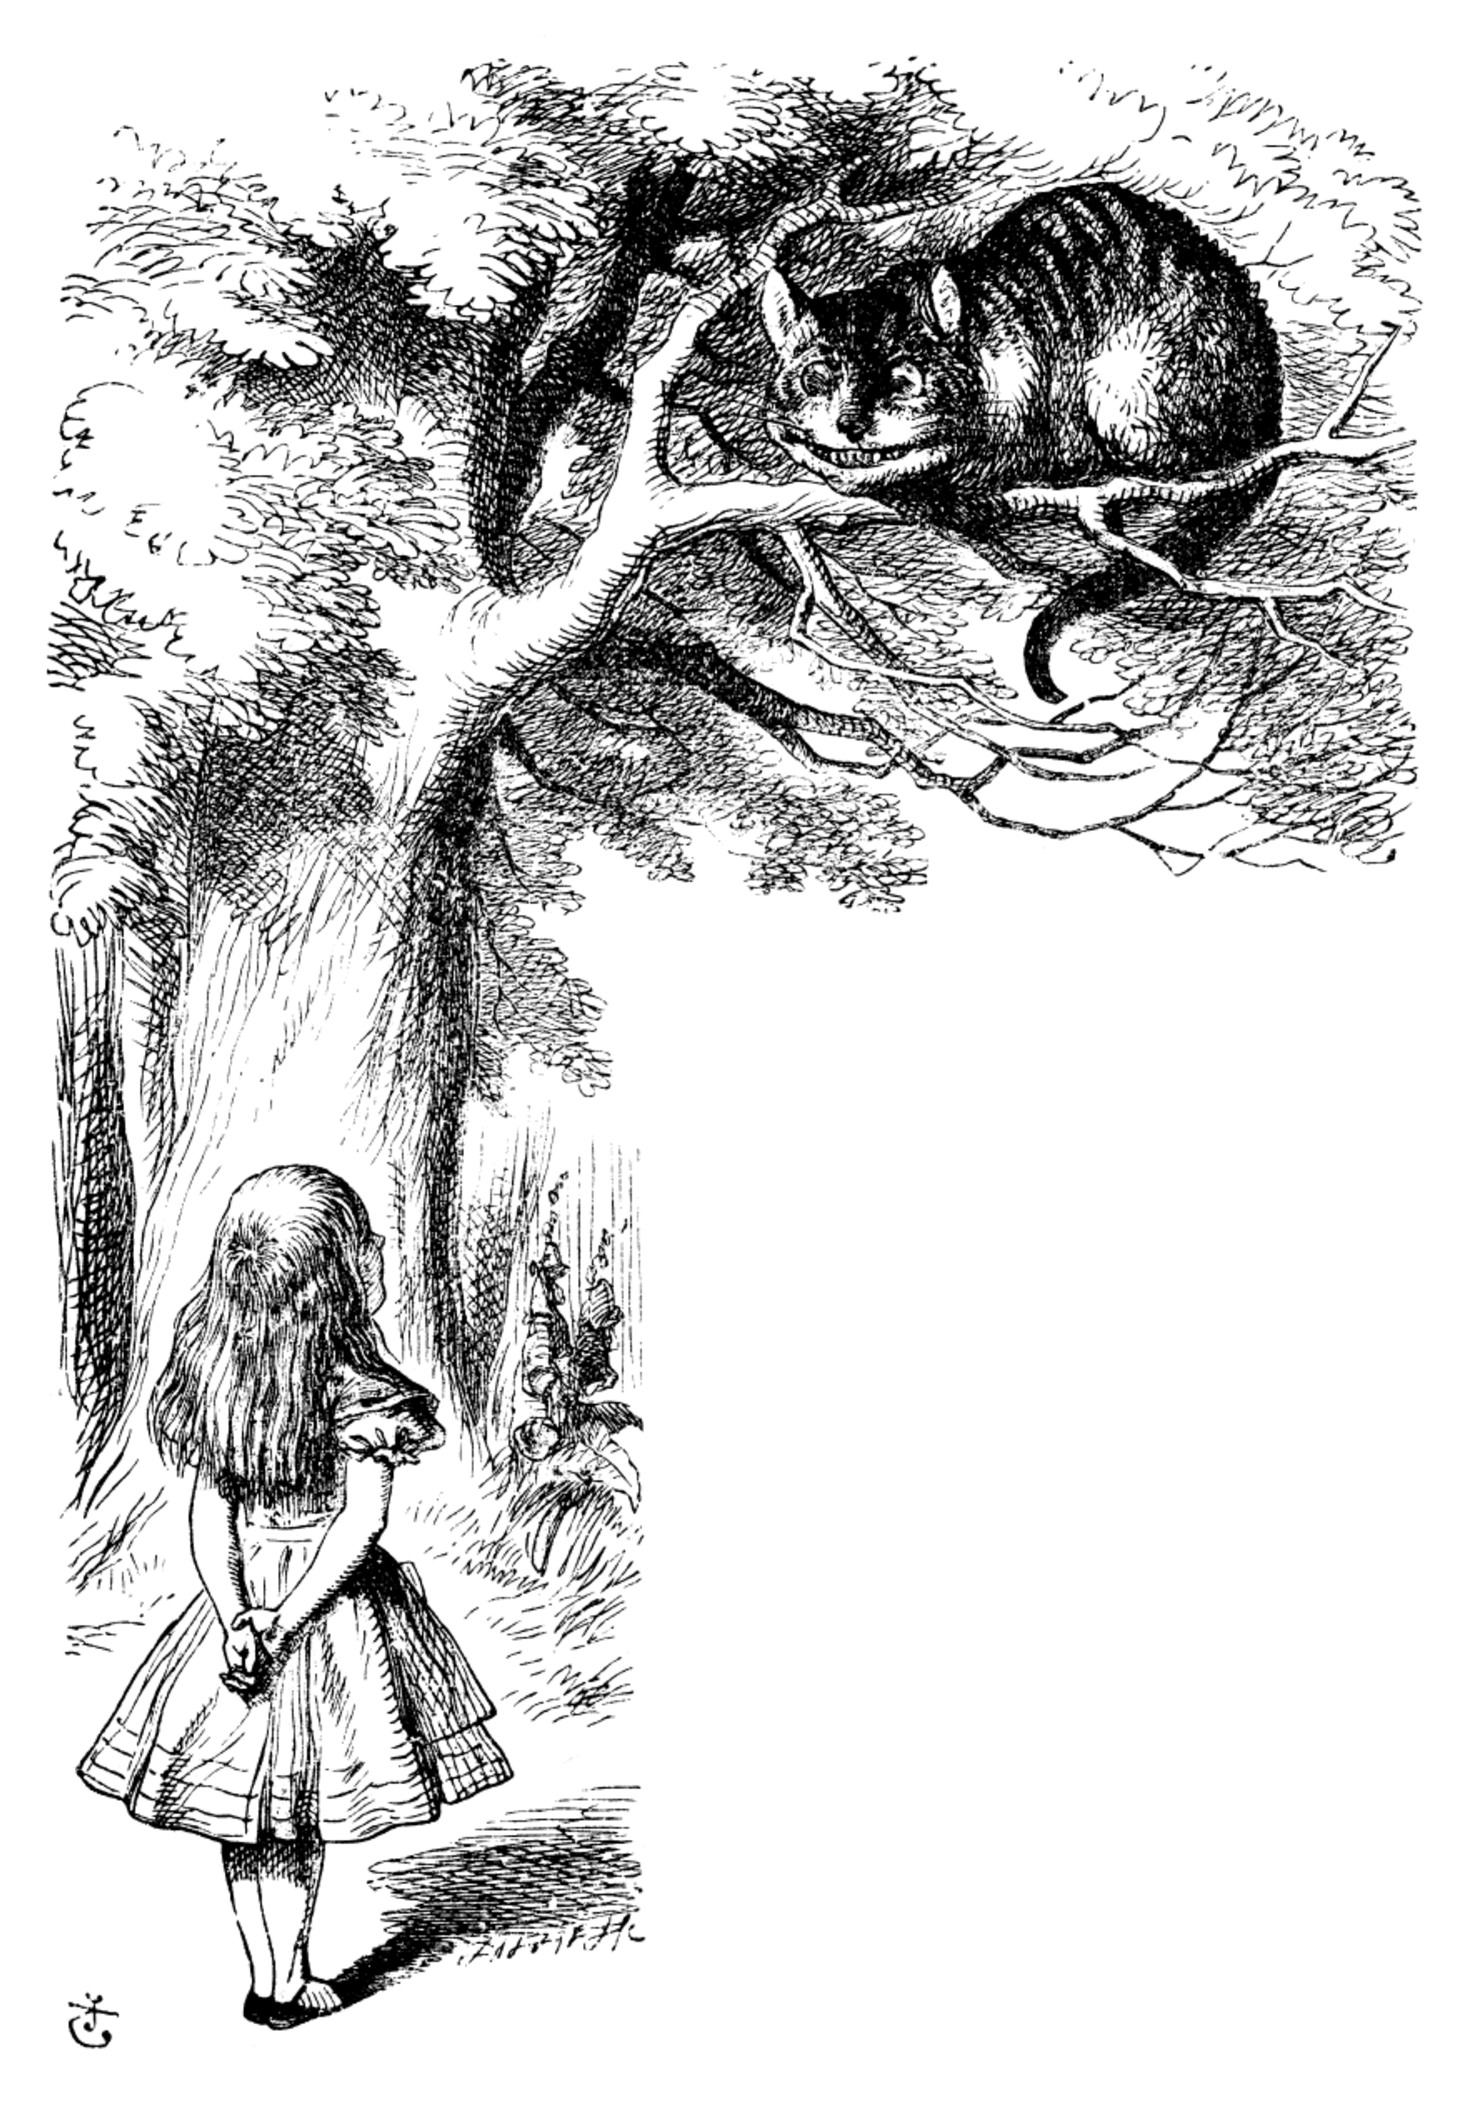
\includegraphics[width=\textwidth]{alice-cheshire}
	\caption[Short figure name.]{This is a full page figure using the FPfigure command. It takes up the whole page and the caption appears on the preceding page. Its useful for large figures. Harvard's rules about full page figures are tricky, but you don't have to worry about it because we took care of it for you. For example, the full figure is supposed to have a title in the same style as the caption but without the actual caption. The caption is supposed to appear alone on the preceding page with no other text. You do't have to worry about any of that. We have modified the fltpage package to make it work. This is a lengthy caption and it clearly would not fit on the same page as the figure. Note that you should only use the FPfigure command in instances where the figure really is too large. If the figure is small enough to fit by the caption than it does not produce the desired effect. Good luck with your thesis. I have to keep writing this to make the caption really long. LaTex is a lot of fun. You will enjoy working with it. Good luck on your post doctoral life! I am looking forward to mine. \label{fig:myFullPageFigure}}
\end{FPfigure}

\lipsum[7-9]

\begin{figure}
    \begin{tikzpicture}
    \node[anchor=south west,inner sep=0] (image) at (0,0,0) 
    {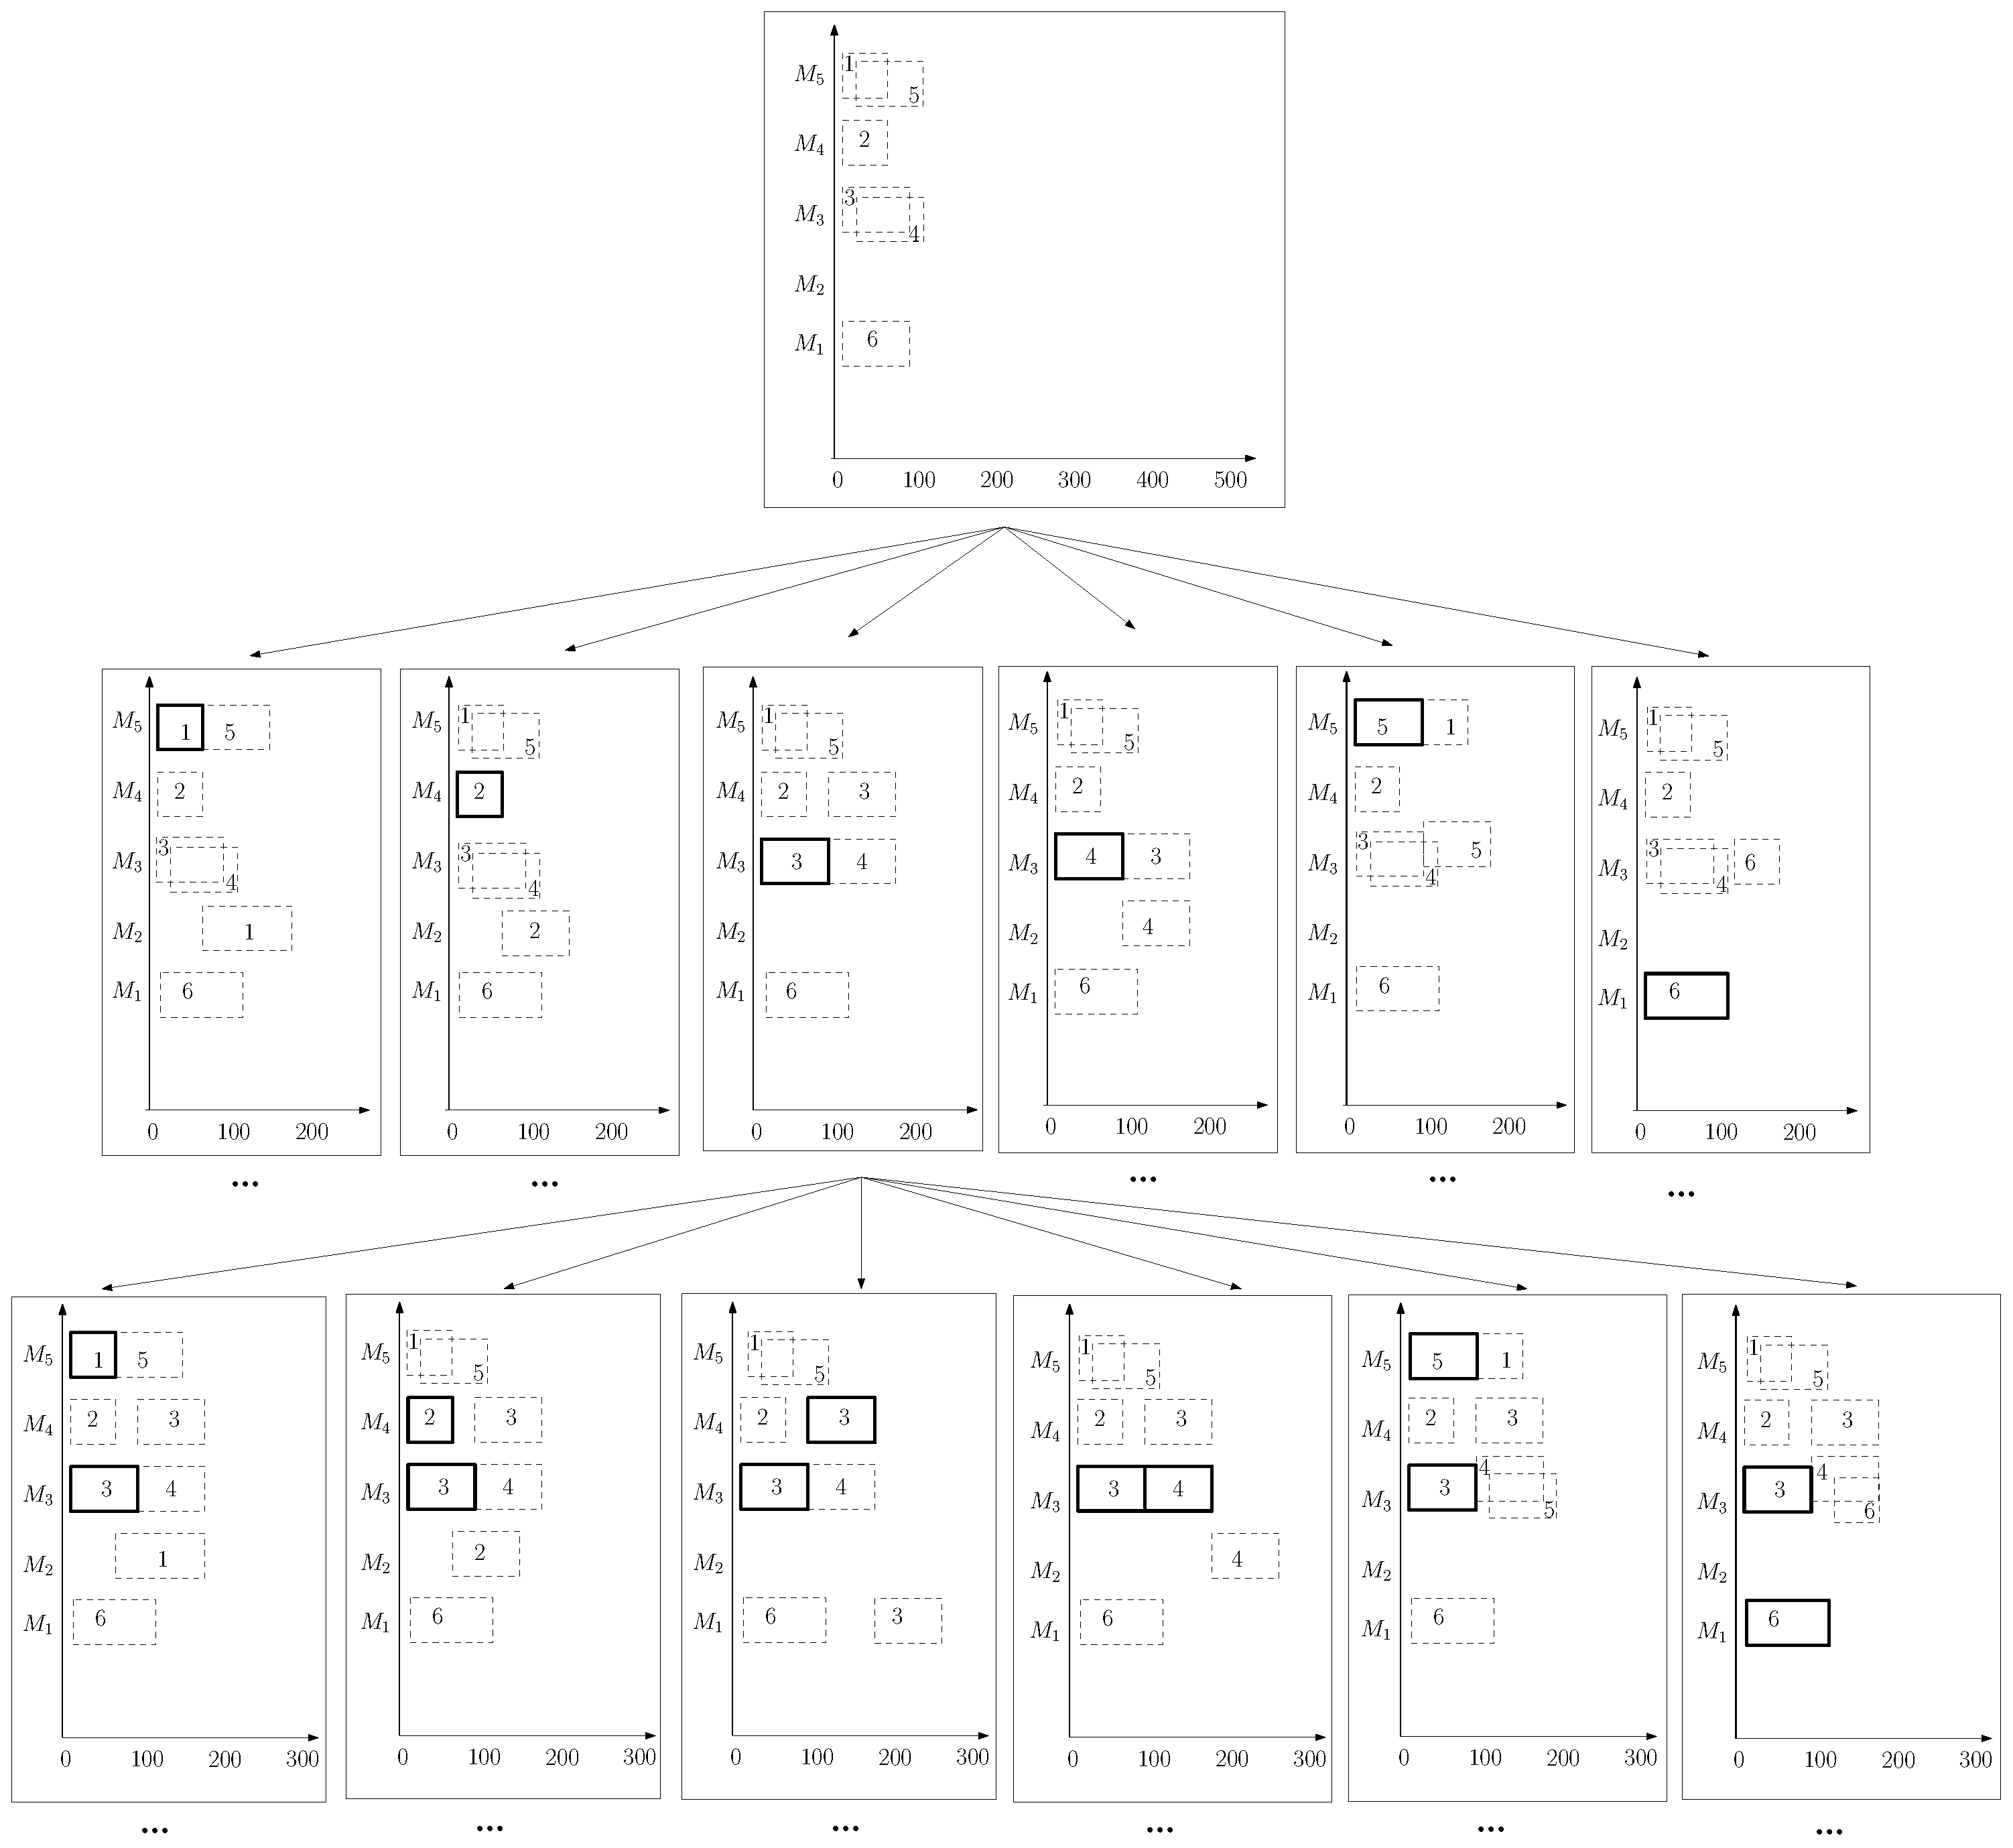
\includegraphics[width=\textwidth]{gametree}};
    \begin{scope}[x={(image.south east)},y={(image.north west)}]
    %% next four lines will help you to locate the point needed by forming a 
    %%grid. comment these four lines in the final picture.↓
    %\draw[help lines,xstep=.1,ystep=.1] (0,0) grid (1,1);
    %\draw[help lines,xstep=.05,ystep=.05] (0,0) grid (1,1);
    %\foreach \x in {0,1,...,9} { \node [anchor=north] at (\x/10,0) {0.\x}; }
    %\foreach \y in {0,1,...,9} { \node [anchor=east] at (0,\y/10) {0.\y};}
    %% upto here↑
    \node (J0) at (0.5,0.71) {};
    \node (J1) at (0.19,0.65) {};
    \node (J2) at (0.42,0.65) {};
    \node (J3) at (0.65,0.65) {};
    \node (J4) at (0.85,0.65) {};
    \draw[-latex] (J0) to[out=-20,in=+20] (J1);
    \draw[-latex] (J0) to[out=-20,in=+20] (J2);
    \draw[-latex] (J0) to[out=-20,in=+20] (J3);
    \draw[-latex] (J0) to[out=-20,in=+20] (J4);
    \node (J4) at (0.82,0.38) {};
    \node (J4J1) at (0.19,0.31) {};
    \node (J4J2) at (0.42,0.31) {};
    \node (J4J3) at (0.65,0.31) {};
    \node (J4J4) at (0.85,0.31) {};
    \draw[-latex] (J4) to[out=-20,in=+20] (J4J1);
    \draw[-latex] (J4) to[out=-20,in=+20] (J4J2);
    \draw[-latex] (J4) to[out=-20,in=+20] (J4J3);
    \draw[-latex] (J4) to[out=-20,in=+20] (J4J4);
    \end{scope}
    \end{tikzpicture}
    \caption{Using tikz over figures}
    \label{fig:tikzoverlay}
\end{figure}

